\section{Calendario delle attività}
In questa sezione vengono presentati i quadri riassuntivi ed i grafici dell'impegno dei ruoli nei diversi periodi. Infine vengono mostrate le incidenze dei vari ruoli nell'intero progetto.

\subsection{Analisi dei Requisiti}
Le ore impiegate in questo periodo sono 195 e vengono ripartite in:
\begin{table}[H]
	\begin{center}
		\begin{tabular}{|c|c|}
			\hline
			\textbf{Ruolo}	& \textbf{Ore} \\
			\hline
			\Res	&	40	\\
			\hline
			\Amm	&	17	\\
			\hline
			\Ana	&	78	\\
			\hline
			\Ver	&	60	\\
			\hline
		\end{tabular}
	\end{center}
	\caption{Ore a ruolo, Analisi dei Requisiti}
\end{table}

\begin{figure}[H]
	\centering
	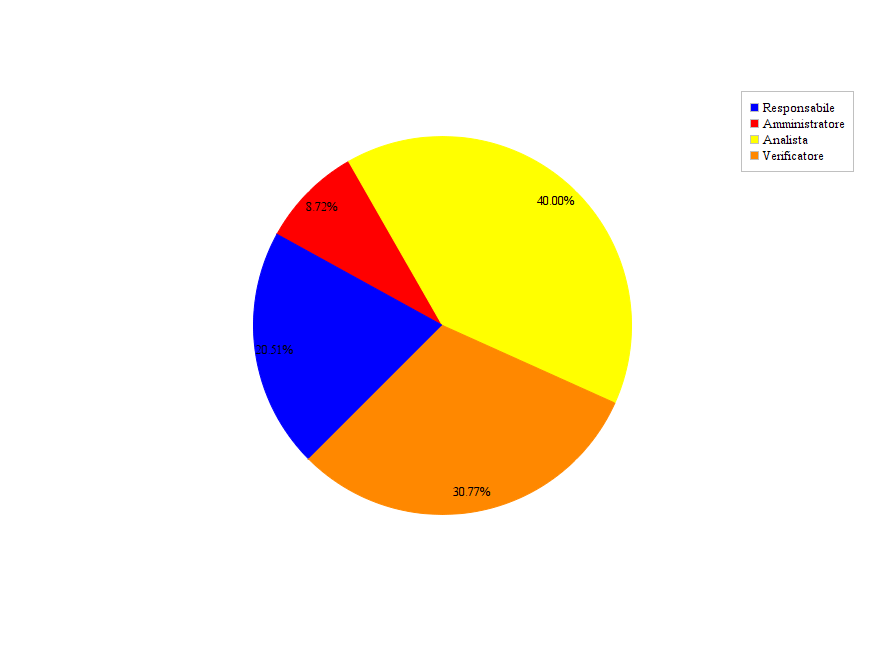
\includegraphics[scale=0.5]{immagini/Grafi/OreRuoloRR}
	\caption{Incidenza ore per ruolo, Analisi dei Requisiti}
\end{figure}

\subsection{Analisi dei Requisiti in Dettaglio}
Le ore impiegate in questo periodo sono 15 e vengono ripartite in:

\begin{table}[H]
	\begin{center}
		\begin{tabular}{|c|c|}
			\hline
			\textbf{Ruolo}	& \textbf{Ore} \\
			\hline
			\Res	&	3	\\
			\hline
			\Amm	&	1	\\
			\hline
			\Ana	&	6	\\
			\hline
			\Ver	&	5	\\
			\hline
		\end{tabular}
	\end{center}
	\caption{Ore a ruolo, Analisi dei Requisiti in Dettaglio}
\end{table}

\begin{figure}[H]
	\centering
	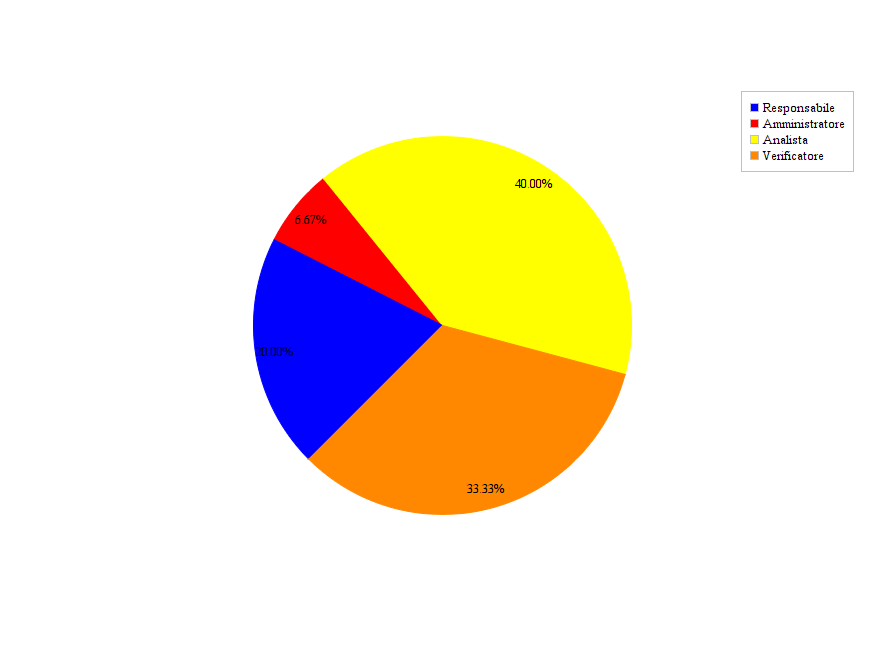
\includegraphics[scale=0.5]{immagini/Grafi/OreRuoloRRD}
	\caption{Incidenza ore per ruolo, Analisi dei Requisiti in Dettaglio}
\end{figure}

\subsection{Progettazione Architetturale}
Le ore totali impiegate in questo periodo sono 225 e vengono ripartite in:
\begin{table}[H]
	\begin{center}
		\begin{tabular}{|c|c|}
			\hline
			\textbf{Ruolo}	& \textbf{Ore} \\
			\hline
			\Res	&	6	\\
			\hline
			\Amm	&	8	\\
			\hline
			\Prog		&	141	\\
			\hline
			\Ver	&	70	\\
			\hline
		\end{tabular}
	\end{center}
	\caption{Ore a ruolo, Progettazione Architetturale}
\end{table}

\begin{figure}[H]
	\centering
	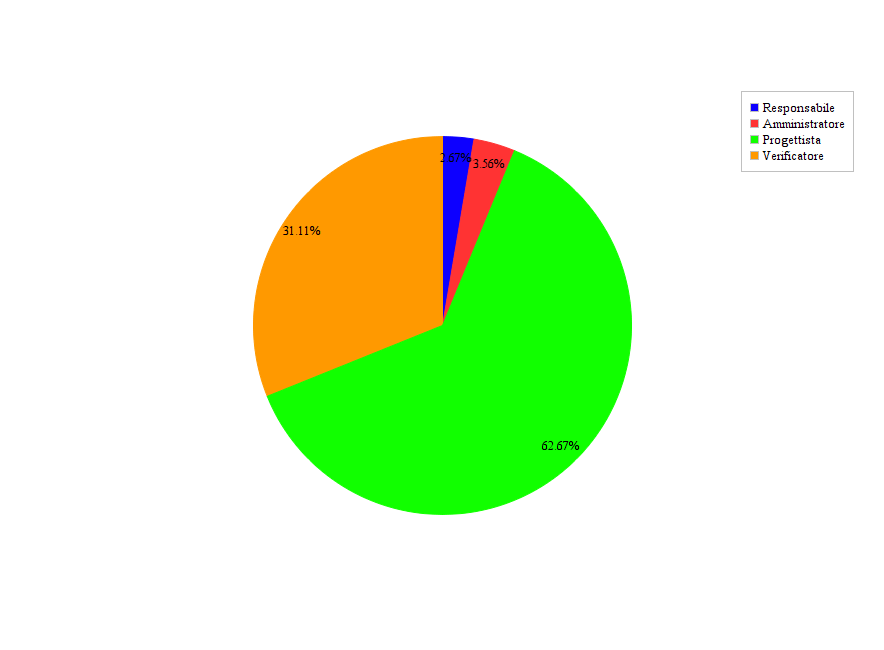
\includegraphics[scale=0.5]{immagini/Grafi/OreRuoloPA}
	\caption{Incidenza ore per ruolo, Progettazione Architetturale}
\end{figure}


\subsection{Progettazione di Dettaglio}
Le ore impiegate in questo periodo sono 140 e vengono ripartite in:
\begin{table}[H]
	\begin{center}
		\begin{tabular}{|c|c|}
			\hline
			\textbf{Ruolo}	& \textbf{Ore} \\
			\hline
			\Res	&	7	\\
			\hline
			\Amm	&	5	\\
			\hline
			\Prog		&	86	\\
			\hline
			\Ver	&	42	\\
			\hline
		\end{tabular}
	\end{center}
	\caption{Ore a ruolo, Progettazione di Dettaglio}
\end{table}

\begin{figure}[H]
	\centering
	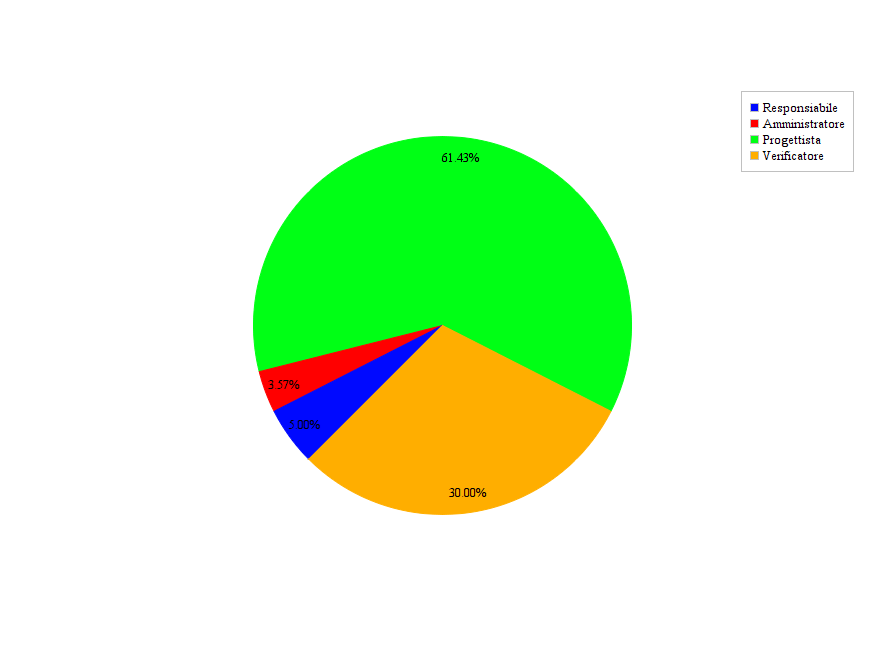
\includegraphics[scale=0.5]{immagini/Grafi/OreRuoloPD}
	\caption{Incidenza ore per ruolo, Progettazione in Dettaglio}
\end{figure}

\subsection{Codifica}
Le ore impiegate in questo periodo sono 248 e vengono ripartite in:
\begin{table}[H]
	\begin{center}
		\begin{tabular}{|c|c|}
			\hline
			\textbf{Ruolo}	& \textbf{Ore} \\
			\hline
			\Res	&	11	\\
			\hline
			\Amm	&	4	\\
			\hline
			\Prog		&	25	\\
			\hline
			\Progr	&	133	\\
			\hline
			\Ver	&	75	\\
			\hline
		\end{tabular}
	\end{center}
	\caption{Ore a ruolo, Codifica}
\end{table}

\begin{figure}[H]
	\centering
	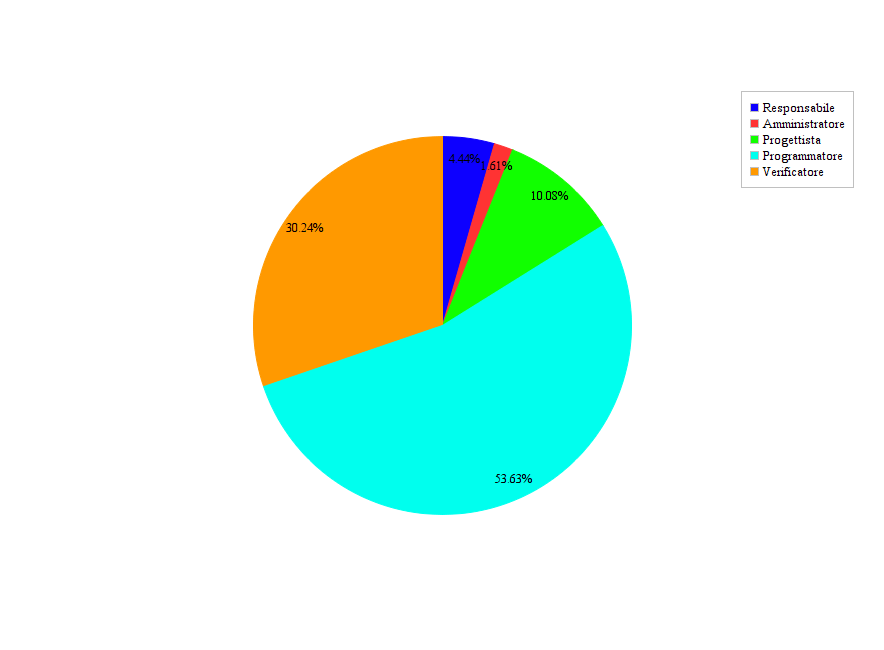
\includegraphics[scale=0.5]{immagini/Grafi/OreRuoloCod}
	\caption{Incidenza ore per ruolo, Codifica}
\end{figure}

\subsection{Validazione}
Le ore totali in questo periodo sono 122 e vengono ripartite in:
\begin{table}[H]
	\begin{center}
		\begin{tabular}{|c|c|}
			\hline
			\textbf{Ruolo}	& \textbf{Ore} \\
			\hline
			\Res	&	9	\\
			\hline
			\Prog		&	20	\\
			\hline
			\Ver	&	93	\\
			\hline
		\end{tabular}
	\end{center}
	\caption{Ore a ruolo, \VV}
\end{table}

\begin{figure}[H]
	\centering
	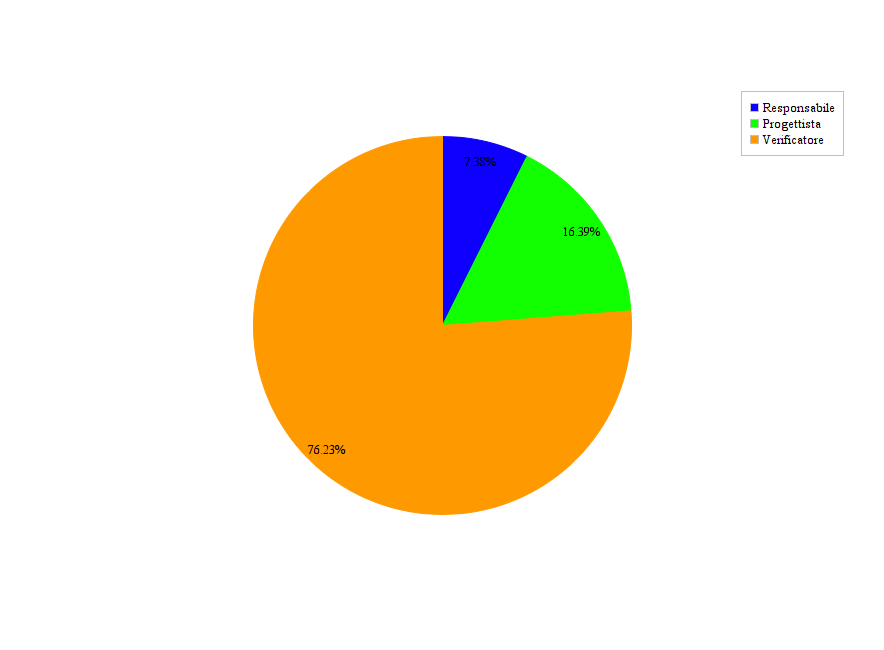
\includegraphics[scale=0.5]{immagini/Grafi/OreRuoloVerifica}
	\caption{Incidenza ore per ruolo, \VV}
\end{figure}

\subsection{Quadro riassuntivo}
Le ore totali del progetto sono 945, di cui 735 remunerabili, così ripartite:
\begin{table}[H]
	\begin{center}
		\begin{tabular}{|c|c|c|}
			\hline
			\textbf{Ruolo}	& \textbf{Ore totali} & \textbf{Ore remunerabili} \\
			\hline
			\Res	&	76	&	33	\\
			\hline
			\Amm	&	35	&	17	\\
			\hline
			\Ana		&	84	&	0	\\
			\hline
			\Prog		&	272	&	272	\\
			\hline
			\Progr	&	133	&	133	\\
			\hline
			\Ver	&	345	&	280	\\
			\hline
		\end{tabular}
	\end{center}
	\caption{Ore a ruolo, Quadro riassuntivo}
\end{table}

\begin{figure}[H]
	\centering
	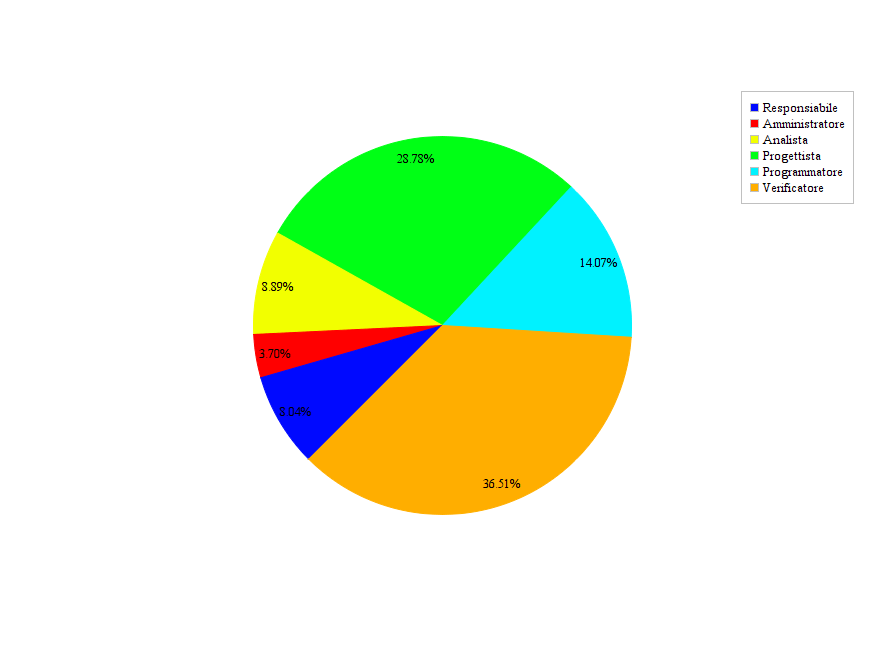
\includegraphics[scale=0.5]{immagini/Grafi/OreRuoloOreTotali}
	\caption{Incidenza ore per ruolo, Ore Totali}
\end{figure}

\begin{figure}[H]
	\centering
	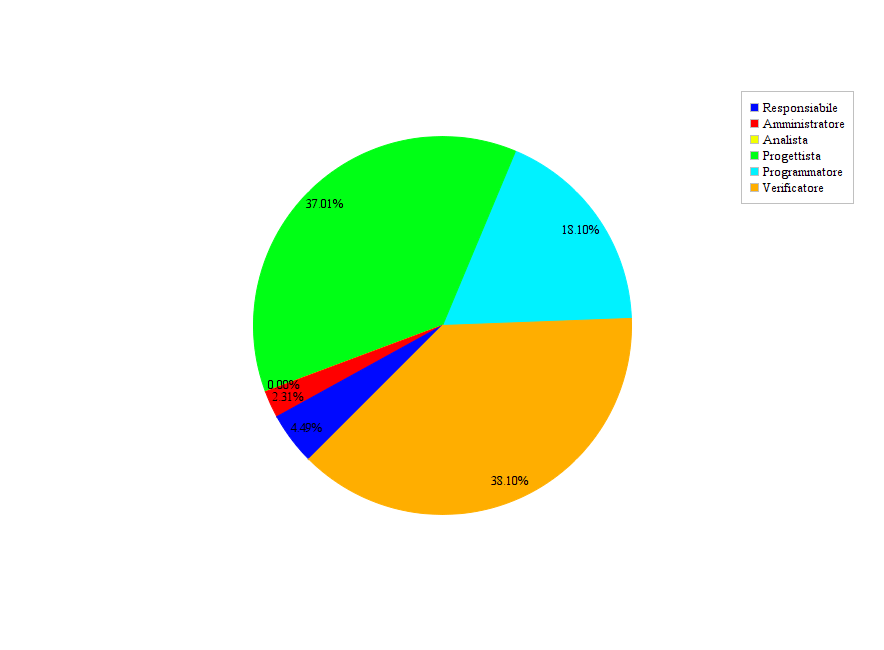
\includegraphics[scale=0.5]{immagini/Grafi/OreRuoloRendicontabili}
	\caption{Incidenza ore per ruolo, Ore Rendicontate}
\end{figure}
